\documentclass[sigconf]{acmart}

% acmart defaults to the ACM Reference Format and includes required metadata.
% Adjust options (e.g., manuscript, review) as needed.
\usepackage{tabularx}
\usepackage{array}
\newcolumntype{Y}{>{\raggedright\arraybackslash}X}
\usepackage{tikz}
\usetikzlibrary{shapes.geometric,arrows.meta,positioning}
\usepackage{listings}
\usepackage{xcolor}
\input{definitions}

\definecolor{tempoBlue}{RGB}{34,54,120}
\definecolor{tempoGray}{RGB}{245,245,245}
\definecolor{tempoGreen}{RGB}{0,96,64}
\definecolor{tempoRed}{RGB}{160,32,32}

\tikzset{tempo/.style={}}

\lstdefinestyle{tempo}{
  language=[Objective]Caml,
  basicstyle=\ttfamily\small,
  keywordstyle=\color{tempoBlue}\bfseries,
  commentstyle=\color{tempoGreen},
  stringstyle=\color{tempoRed},
  backgroundcolor=\color{tempoGray},
  frame=single,
  framerule=0pt,
  rulecolor=\color{tempoGray},
  linewidth=\columnwidth,
  xleftmargin=0pt,
  xrightmargin=0pt,
  framexleftmargin=1mm,
  framexrightmargin=1mm,
  framesep=2mm,
  aboveskip=10pt,
  belowskip=8pt,
  breaklines=true,
  showstringspaces=false,
  columns=fullflexible
}

\title{\tempo{}: Effect-Based Synchronous Reactive Control in OCaml}

\author{Fr\'ed\'eric Dabrowski}
\affiliation{%
  \institution{Univ. Orl\'eans, INSA Centre Val de Loire, LIFO EA 4022}
  \city{Orl\'eans}
  \country{France}
}
\email{frederic.dabrowski@univ-orleans.fr}

\begin{document}

\begin{abstract}
\tempo{} is a lightweight synchronous runtime for OCaml that revisits the
reactive control lineage of Esterel, FairThreads, and ReactiveML using OCaml
5.3 algebraic effects. The library implements logical instants, valued signals,
guards, and weak preemption while preserving the delayed-absence discipline
that enables deterministic concurrency under standard purity assumptions (no
shared mutable state dependent on intra-instant order and order-insensitive
aggregation). This report positions \tempo{} in its
semantic context, explains its API and usage patterns, and provides a detailed
account of how effect handlers realize the scheduler and control primitives at
library level. The current draft emphasizes design and implementation; formal
correctness and quantitative evaluation are identified as future work.

\end{abstract}

\keywords{tempo, ocaml, synchronous, reactive control, algebraic effects}

\maketitle

\section{Introduction}
Reactive systems must continuously respond to an environment, often under
strict timing and safety constraints. Programming such systems is difficult
because concurrency, external events, and state updates interact in ways that
can break determinism. Ad-hoc callback-based designs are common, but they make
control flow implicit and complicate reasoning about ordering, causality, and
reproducibility.

Synchronous reactive programming addresses these challenges by discretizing
time into logical instants and by defining what is observable at instant
boundaries. A classic distinction is between control-flow and dataflow
approaches: Esterel represents the control-flow lineage, while Lustre
represents the dataflow lineage \cite{esterel1992,lustre1991}. In both cases,
logical instants enable deterministic behavior and rigorous analyses of
causality and scheduling. Survey discussions situate these languages within a
shared semantic framework \cite{benveniste2003}.

These synchronous languages achieve high assurance by imposing restrictions
that permit static scheduling and causality checks. The restrictions make it
possible to decide properties such as determinism and absence/presence
consistency, but they also limit expressiveness when integrated with richer
general-purpose languages.

The key semantic question is when signal absence can be observed. In Esterel,
absence is decided within the instant, enabling static scheduling but
restricting dynamic behavior \cite{esterel1992}. Boussinot's FairThreads model
defers absence observation to instant end, allowing more flexible composition
while preserving determinism \cite{fairthreads2003}. From a programmer's
perspective, each instant follows a two-phase discipline: react while tasks run
and signals may become present, then finalize when the instant quiesces and
absence becomes observable.
This distinction is central because it determines which control patterns are
expressible without sacrificing determinism.
Subsequent work revisits the synchronous model inside richer language settings.
On the control-flow side, ReactiveML adapts Esterel-style signals and the
synchronous hypothesis to a higher-order language \cite{reactiveml2005}. On the
dataflow side, FRP explores declarative, time-varying values with different
operational priorities \cite{frp1997}. 

This paper introduces \tempo{}: a library that revisits ReactiveML's control-flow
model using OCaml 5.3 algebraic effects as its implementation mechanism. \tempo{}
follows the delayed-absence discipline introduced by Boussinot's FairThreads,
which ReactiveML also adopts, and brings this approach to a modern OCaml
runtime without modifying the compiler \cite{fairthreads2003,reactiveml2005}.
\tempo{} re-implements the core control constructs (signals, guards, weak
preemption) as a pure library. It executes programs in discrete logical
instants: signals can be emitted and tasks can run within an instant, but the
\emph{absence} of a signal is only observable at the end of the instant. This
article presents \tempo{} as a reactive control runtime and explains its design
choices and effect-based implementation in OCaml 5.3. It does not attempt a
formal semantics or a quantitative evaluation, and focuses instead on the
design rationale, API, and implementation details needed to motivate future
formalization. Determinism is discussed under standard purity assumptions:
programs should avoid shared mutable state whose outcomes depend on
intra-instant scheduling, and aggregate combine functions should be
order-insensitive. These assumptions match the synchronous control model and
are stated explicitly in the core constructs section.
\begin{itemize}
\item A library-level formulation of synchronous reactive control in OCaml,
  positioned within the Esterel/FairThreads/ReactiveML lineage.
\item An implementation account of how algebraic effects realize signals,
  guards, suspension, and weak preemption.
\item End-to-end examples that illustrate standard synchronous control idioms
  using the \tempo{} API.
\end{itemize}

\section{Boussinot's Reactive Control Model}
\label{sec:boussinot-control}
Boussinot's reactive control model organizes concurrency around logical
instants. Execution proceeds as a sequence of reaction cycles: within an
instant, all runnable activities execute until they suspend or the system
quiesces, and only after that quiescence can absence be observed. This notion
of instant provides a global time base that makes reactions comparable and
deterministic at instant boundaries \cite{fairthreads2003}.

\paragraph{Signals (unvalued)}
To simplify the presentation, we consider unvalued signals. A signal is either
present or absent for the entire duration of an instant. When a signal is
emitted, it becomes present for all components; when it is not emitted, it
remains absent for all components. The effective order of emissions within the
instant must not affect the observable behavior: presence is a global property
for the instant, not a per-thread event. This makes synchronization explicit
and avoids order-sensitive communication.

\paragraph{Suspension}
Threads are cooperative: they execute until they reach a suspension point and
then yield control. Suspension can be explicit (e.g., waiting for a signal or
for the next instant). The key property is that suspension preserves the
instant structure: a suspended thread resumes only at a well-defined instant
boundary or when a relevant signal becomes present.

\paragraph{Algorithmic view (abstract)}
We use a small algorithmic notation that mirrors Boussinot's control vocabulary.
Behaviors (threads) are composed from a core set of control operators. The
notation hides values when they are not essential to control and uses abstract
behaviors inside control structures:
\begin{lstlisting}[style=tempo]
(* Abstract control language; B is an abstract behavior. *)
B ::= skip
    | emit s          (* mark signal s present in current instant *)
    | await s         (* resume at next instant where s is present *)
    | pause           (* resume at the next instant *)
    | B1; B2          (* sequence *)
    | parallel [B1; ...; Bn]
    | when s do B     (* guard: block until s is present *)
    | watch s do B    (* weak preemption: stop B after this instant if s emits *)
\end{lstlisting}

The constructs are interpreted at instant boundaries. \texttt{emit s} makes
\texttt{s} present for the remainder of the instant. \texttt{await s} suspends
until the next instant where \texttt{s} is present, while \texttt{pause} always
advances to the next instant. In \texttt{when s do B}, the guard is a blocking
condition: if \texttt{s} is absent, the entire behavior suspends and can only
resume at a future instant where \texttt{s} is present. In \texttt{watch s do B},
the body \texttt{B} runs normally in the current instant, but if \texttt{s} is
emitted during that instant, \texttt{B} is not allowed to continue into the next
instant (weak preemption).

This abstract view lets us express control patterns without committing to a
concrete evaluation order. For example, \texttt{when s do \{B1; B2\}} denotes an
entire guarded behavior, and \texttt{watch s do \{parallel [B1; B2]\}} denotes a
preemptible concurrent block.

\paragraph{Micro-examples (abstract)}
\begin{lstlisting}[style=tempo]
(* Suspension across instants *)
emit s; pause; await s

(* Guarded behavior: runs only if s is present *)
when s do (emit out)

(* Weak preemption: body stops after instant if k is emitted *)
watch k do (emit tick; pause; emit tick)

(* Disjunctive enabling via parallel guards *)
parallel [
  (when g1 do B);
  (when g2 do B)
]
\end{lstlisting}

\paragraph{Preemption and Esterel}
Control languages such as Esterel rely on preemption to enforce control
structure. In Boussinot's setting, preemption is \emph{weak}: if a preempting
signal is emitted in instant $t$, a preempted computation may complete its
current instant but must not continue into $t{+}1$. The alternative would be
\emph{strong} preemption, where a computation is stopped immediately within
the same instant. Weak preemption is the appropriate choice here because the
model treats the instant as an atomic reaction: all threads share the same
present/absent view for the whole instant, and mid-instant interruption would
reintroduce order dependence and break determinism \cite{esterel1992,fairthreads2003}.

This model yields a control-centric view of concurrency: threads cooperate,
rendezvous on signal presence, and advance in lockstep from one instant to the
next. \tempo{} adopts this discipline as the semantic baseline for its runtime.

\paragraph{From FairThreads to ReactiveML (abstract view)}
ReactiveML lifts this control model into a higher-order ML setting while
preserving the delayed-absence discipline. It exposes a small set of reactive
operators---\texttt{signal}, \texttt{emit}, \texttt{await}, \texttt{pause},
\texttt{when}, and \texttt{watch}---that directly encode the instant-based
control structure. These constructs compile to a runtime that enforces the
instant discipline and yields deterministic behavior at instant boundaries,
while allowing higher-order composition over reactive processes
\cite{reactiveml2005}.

At the same level of abstraction, this places ReactiveML in the control-flow
lineage (Esterel/FairThreads), in contrast to dataflow approaches such as FRP
that emphasize time-varying values and stream composition \cite{frp1997}.
Recent FRP work has refined operational guarantees such as causality and space
usage (e.g., \cite{perez2016frp,bahr2019ratt,bahr2022modalfrp,bahr2023async}),
but these advances are orthogonal to the control-centric lineage considered
here.

ReactiveML also benefits from language-level integration: its compiler can
enforce discipline constraints and optimize the scheduling structure
statically. \tempo{} chooses a different point in the design space by reusing
OCaml 5.3 algebraic effects to recover similar control constructs as a
library. This enables straightforward embedding in existing OCaml codebases
while leaving stronger static guarantees to future work.

\section{ReactiveML Context and Core Constructs}
ReactiveML is the closest language-level incarnation of the control model
described in Section~\ref{sec:boussinot-control}. It offers dedicated syntax,
compiler support, and a runtime tailored to instants and delayed absence
\cite{reactiveml2005}. We do not reproduce the language itself here; instead,
we use it as a point of reference for the library-based approach of \tempo{}.

The remainder of this section therefore focuses on the core control constructs
and their synchronous properties, as they appear in \tempo{}'s library API.
\tempo{} exposes a small set of constructs that mirror the common vocabulary of
reactive control languages. Signals are the primary communication medium within
an instant. A signal is either present or absent during an instant; presence is
established by emission, while absence can only be observed at the end of the
instant. This delayed observation is central to deterministic behavior.

\paragraph{Semantic contract (informal)}
\tempo{} guarantees determinism at instant boundaries: for a fixed input stream,
the set of signals present at each instant and the values delivered to awaiters
are deterministic. What is not specified is the internal evaluation order of
tasks within an instant; relying on that order can break determinism when using
shared mutable state. The semantics therefore define \emph{what} is observable
per instant, not the precise scheduling order inside it.
We use \emph{instant boundary} and \emph{end of the instant} interchangeably.

\paragraph{Non-guarantees}
\tempo{} does not guarantee deterministic outcomes when programs depend on the
intra-instant evaluation order or shared mutable state (e.g., reference cells).
Such behaviors are outside the semantic contract and must be avoided or
controlled by static analyses.

\paragraph{Minimal vocabulary}
\begin{itemize}
\item \textbf{Instant}: logical time step where reactions occur.
\item \textbf{Presence/absence}: a signal is present if emitted in the instant.
\item \textbf{Guard}: a condition that blocks a task until a signal is present.
\item \textbf{Weak preemption}: termination at the end of the instant.
\item \textbf{Determinism}: observables per instant are uniquely determined by inputs.
\end{itemize}

\paragraph{Determinism statement (informal)}
Let $I$ be a fixed input sequence per instant. \tempo{} guarantees that, for each
instant $t$, the multiset of event-signal emissions and the values returned by
\texttt{await} and \texttt{await\_immediate} are uniquely determined by $I$,
assuming programs avoid shared mutable state that depends on intra-instant
ordering and aggregate combine functions are pure and order-insensitive. No
guarantee is made about the relative order of tasks within an instant.
\paragraph{Observable vs non-observable (summary)}
\begin{itemize}
\item \textbf{Observable:} which signals are present at each instant boundary,
  and the values delivered to \texttt{await} and \texttt{await\_immediate}.
\item \textbf{Not observable:} the order in which tasks run within the instant,
  or the ordering of side effects on shared mutable state.
\end{itemize}
\paragraph{Aggregate signals and \texttt{await\_immediate}}
Aggregate signals are delivered only at instant end; thus their determinism is
defined by the combined value, not by the order of emissions within the instant.
\texttt{await\_immediate} is restricted to event signals, which allows safe
same-instant resumption without introducing ambiguity in the delivered value.
For deterministic aggregation, the combine function should be pure and
order-insensitive (associative/commutative), since the intra-instant order of
emissions is not part of the semantics.

\paragraph{Observable trace (informal)}
An execution can be summarized by a per-instant trace $au(t)$ that records:
\begin{itemize}
\item \textbf{Event signals:} the unique value emitted in instant $t$, or
  \emph{absent} if no emission occurs.
\item \textbf{Aggregate signals:} the combined value delivered at instant end
  (or the initial accumulator if no emission occurred).
\item \textbf{Outputs:} values emitted on the output signal at instant end.
\end{itemize}
The trace intentionally omits intra-instant scheduling order. Two runs are
observationally equivalent if they produce the same $au(t)$ for all $t$.

\paragraph{\texttt{await} vs \texttt{await\_immediate}}
\texttt{await} always resumes at the next instant, even if the signal is already
present. If the event signal is present, \texttt{await\_\allowbreak immediate}
may resume in the current instant. This can be useful for immediate reactions,
but it is restricted to event signals to preserve determinism.

\begin{figure}[h]
\centering
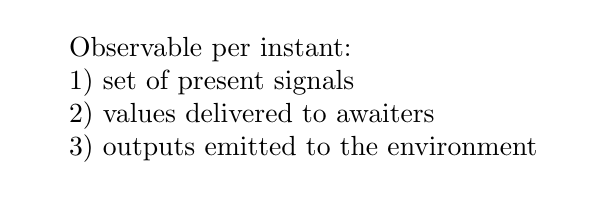
\begin{tikzpicture}[
  box/.style=tempo,
  draw,
  rounded corners,
  align=left,
  minimum width=70mm,
  minimum height=8mm
]
\node[box] {
Observable per instant:\\
1) set of present signals\\
2) values delivered to awaiters\\
3) outputs emitted to the environment
};
\end{tikzpicture}
\caption{Observables that define determinism at instant boundaries.}
\end{figure}

\paragraph{Determinism in action}
For the same input stream, the observables above do not change. For example,
if the host emits input \texttt{1} at instant $t$ and \texttt{2} at instant
$t{+}1$, then the program below deterministically emits \texttt{1} at $t{+}1$
and \texttt{2} at $t{+}2$.
\begin{lstlisting}[style=tempo]
let program input output =
  let v = await input in
  emit output v
\end{lstlisting}

\begin{table}[h]
\centering
\begin{tabularx}{\linewidth}{lY}
\hline
Instant & Observable events \\ \hline
$t$ & input emits \texttt{1}; no output yet. \\
$t{+}1$ & output emits \texttt{1}; input emits \texttt{2}. \\
$t{+}2$ & output emits \texttt{2}. \\ \hline
\end{tabularx}
\caption{Timeline for the simple echo program.}
\end{table}

\paragraph{Mini-specification (informal)}
The behavior of a program can be described per instant:
\begin{enumerate}
\item At instant start, all signals are absent.
\item Emissions during the instant mark signals present; event signals accept
  at most one emission.
\item \texttt{await} resumes at the next instant; \texttt{await\_immediate}
  may resume in the current instant for event signals already present.
\item Absence is observed only at instant end; guard rechecks occur at the next
  instant.
\end{enumerate}

\paragraph{Intuitive timeline}
Consider two instants with a single signal \texttt{s}. In instant $t$, a task
emits \texttt{s} and another task awaits it. The awaiting task can only resume
at the \emph{beginning} of instant $t{+}1$, because the presence of \texttt{s}
becomes observable only after the instant ends. If \texttt{s} is never emitted
in instant $t$, that absence is observable only at the end of $t$, and a
guarded task can only retry in instant $t{+}1$. Observable events are therefore
the set of signals present at instant boundaries, not intermediate scheduling
steps within the instant.

Emissions mark a signal as present and provide a value. \tempo{} supports two
signal kinds: event signals accept at most one emission per instant, while
aggregate signals combine multiple emissions through an associative folding
function. Suspension is expressed through \texttt{await}, which resumes at the
beginning of the next instant, and \texttt{await\_immediate}, which may resume
in the current instant if an event signal is already present.

Guards and preemption encode control flow. Guarded execution activates a
behavior only when a guard signal becomes present. Weak preemption terminates a
behavior at the end of the current instant after a preempting signal is
emitted, allowing other concurrent tasks to observe the emission within the
same instant. These constructs preserve determinism by maintaining a single
global notion of instants and deferring absence decisions to instant boundaries.
The distinction between strong and weak restart patterns is often encoded by
explicit pauses: inserting a \texttt{pause} between successive activations
ensures that a reaction cannot retrigger within the same instant, which matches
the weak restart discipline commonly used in synchronous control.

Guarded execution is \emph{blocking}, so a sequential nesting of \texttt{when\_}
does not implement a disjunction. A disjunction is obtained by running
multiple guarded branches in parallel, each able to unblock independently.
Similarly, nested \texttt{watch} constructs compose as disjunctions: a body is
preempted if any watched signal is emitted in the current instant. This is
consistent with the control interpretation where multiple guards or preemption
sources represent alternative enabling or disabling conditions.

\begin{lstlisting}[style=tempo]
(* Disjunction of guards: run guarded branches in parallel. *)
parallel [
  (fun () -> when_ g1 (fun () -> body ()));
  (fun () -> when_ g2 (fun () -> body ()));
];

(* Disjunction of preemption: stop when s1 or s2 is emitted. *)
watch s1 (fun () -> watch s2 (fun () -> body ()))
\end{lstlisting}

\section{\tempo{} Overview}
\tempo{} is a lightweight synchronous runtime for OCaml. It adopts the delayed
absence principle of FairThreads and ReactiveML, but implements it entirely at
library level using OCaml 5.3 algebraic effects. Programs execute over a
sequence of logical instants, interact via valued signals, and compose
concurrently under a deterministic scheduler.

The runtime preserves the core control semantics: signal presence is decided
within the instant, absence is observed only at instant end, and preemption is
weak and instant-aligned. The key design choice is to encode these constructs
as effectful operations interpreted by handlers. This keeps the model explicit
in user code and avoids changes to the language runtime, while still enabling
expressive control operators and a clear mapping to synchronous concepts.

Compared to ReactiveML, \tempo{} trades language-level syntax and compilation
support for a pure library approach based on OCaml 5.3 effects, making it
easier to embed into existing codebases and to experiment with scheduling.

\paragraph{Programming model}
\tempo{} programs are written as ordinary OCaml functions that receive two
signals: an input signal provided by the host and an output signal used to
publish results at the end of each instant. Instants are advanced by the
\texttt{execute} loop, which invokes host hooks before and after each instant.
Signals are first-class values, so they can be stored in data structures,
returned from functions, and passed between components.

\paragraph{Determinism and control}
Determinism is defined at instant boundaries: given the same input emissions,
the observable outputs at each instant are fixed, regardless of internal task
interleavings. Within an instant, the scheduler runs tasks in a fixed order,
but the semantics does not expose this ordering, which keeps the model
declarative from the user's perspective.

\paragraph{Design rationale}
\tempo{} adopts algebraic effects for three reasons. First, effects provide
first-class, delimited continuations, which allow the scheduler to control
resumption points precisely. Second, a library-level approach avoids modifying
the OCaml compiler and keeps integration friction low. Third, handlers make the
control flow explicit in user space, which simplifies experimentation with
scheduling policies and debugging.

\paragraph{Non-goals (current scope)}
\tempo{} does not attempt to provide static guarantees (e.g., single-emission
checks or determinism proofs) and does not perform compilation into automata.
These choices keep the library small and explainable, but they also motivate
the future work discussed in Section~\ref{sec:future-work}.

\section{Public API}
\tempo{} exposes a small API centered on signals, instants, and control
combinators. The API can be grouped into three layers: signal creation and
manipulation, control flow within instants, and execution of a complete
reactive program.

\paragraph{Signal types}
\tempo{} uses two signal families:
\begin{itemize}
\item \texttt{'a signal}: event signal carrying values of type \texttt{'a}.
  At most one emission is allowed per instant.
\item \texttt{('emit, 'agg) agg\_signal}: aggregate signal that can receive
  multiple emissions of type \texttt{'emit} per instant, folded into a value
  of type \texttt{'agg} using a user-provided combine function.
\end{itemize}

\paragraph{Informal type signatures}\mbox{}\\
\begin{itemize}
\item \texttt{new\_signal : unit -> 'a signal}
\item \texttt{new\_signal\_agg : initial:'agg -> combine:('agg -> 'emit -> 'agg) -> ('emit, 'agg) agg\_signal}
\item \texttt{emit : 'a signal -> 'a -> unit}
\item \texttt{await : 'a signal -> 'a}
\item \texttt{await\_immediate : 'a signal -> 'a}
\item \texttt{pause : unit -> unit}
\item \texttt{when\_ : 'a signal -> (unit -> unit) -> unit}
\item \texttt{watch : 'a signal -> (unit -> unit) -> unit}
\item \texttt{parallel : (unit -> unit) list -> unit}
\item \texttt{fork : (unit -> unit) -> thread}
\item \texttt{join : thread -> unit}
\item \texttt{execute : ('a signal -> 'b signal -> unit) -> unit}
\end{itemize}
These signatures are indicative; see \texttt{Tempo} for precise types.

\paragraph{Signal creation and communication}\mbox{}\\
\begin{itemize}
\item \texttt{new\_signal ()} creates an event signal.
\item \texttt{new\_signal\_agg extasciitilde initial extasciitilde combine}
  creates an aggregate signal with an initial accumulator and a combine
  function.
\item \texttt{emit signal value} marks a signal present in the current instant
  and delivers \texttt{value}.
\item \texttt{await signal} suspends the current task until the signal becomes
  present, resuming at the beginning of the next instant with the signal
  value.
\item \texttt{await\_immediate signal} resumes in the same instant if the signal
  is already present. To preserve determinism, it is restricted to event
  signals.
\end{itemize}
\begin{lstlisting}[style=tempo]
let s = new_signal ()
emit s 1
let v = await s
\end{lstlisting}

Aggregate signals support accumulation across multiple emissions in the same
instant:
\begin{lstlisting}[style=tempo]
let s = new_signal_agg
  ~initial:0
  ~combine:(fun acc x -> acc + x)
emit s 1;
emit s 2;
let sum = await s
\end{lstlisting}
Contract. The combine function should be pure and ideally associative and
commutative; otherwise the aggregate result may depend on the intra-instant
evaluation order, which is not specified by the semantics. If no emission
occurs during an instant, the value delivered is the initial accumulator.

\paragraph{Control flow and concurrency}\mbox{}\\
\begin{itemize}
\item \texttt{pause ()} suspends the current task until the next instant.
\item \texttt{parallel [p1; \dots; pn]} executes a list of behaviors
  synchronously within the same instant.
\item \texttt{when\_ guard body} executes \texttt{body} only if \texttt{guard} is
  present; otherwise the task is blocked until the guard becomes present.
\item \texttt{watch signal body} executes \texttt{body} and terminates it at the
  end of the instant in which \texttt{signal} is emitted (weak preemption).
\item \texttt{fork} and \texttt{join} create and synchronize logical threads.
\end{itemize}
\begin{lstlisting}[style=tempo]
parallel [
  (fun () -> emit s 1);
  (fun () -> pause (); emit s 2)
]
watch s (fun () ->
  when_ s (fun () -> emit s 3))
\end{lstlisting}

Usage notes:
\begin{itemize}
\item Event signals enforce single emission per instant; aggregate signals are
  designed for multi-producer scenarios.
\item \texttt{await} always resumes in the next instant, while
  \texttt{await\_immediate} can resume in the current instant if the signal is
  already present.
\item \texttt{parallel} defines a logical concurrency scope; \texttt{fork} and
  \texttt{join} are useful when a thread handle is needed.
\end{itemize}

\paragraph{Execution entry point}\mbox{}\\
\texttt{execute} runs a program over instants. It accepts optional
\texttt{input} and \texttt{output} hooks to interact with the environment by
injecting values into an input signal and observing an output signal at each
step. Inputs are injected at the beginning of each instant; outputs are
observed at the end of the instant after the scheduler reaches quiescence. The
program is expressed as a function that receives these two signals and defines
the reactive behavior.
\begin{lstlisting}[style=tempo]
execute (fun input output ->
  let v = await input in
  emit output v)
\end{lstlisting}

\paragraph{Low-level API}
The \texttt{Tempo.Low\_level} module exposes explicit termination and
thread-control primitives. It is intended for advanced uses, such as building
custom control operators that are not directly provided by the high-level API.

\paragraph{Summary table}
\begin{table}[h]
\centering
\begin{tabularx}{\linewidth}{lY}
\hline
Item & Role and constraints \\ \hline
\texttt{'a signal} & Event signal; at most one emission per instant. \\
\texttt{('e,'a) agg\_signal} & Aggregate signal; combine multiple emissions. \\
\texttt{emit} & Mark present; event signals accept a single emit per instant. \\
\texttt{await} & Suspend to next instant; resumes with signal value. \\
\texttt{await\_immediate} & Same-instant await; event signals only. \\
\texttt{pause} & Suspend until next instant. \\
\texttt{when\_} & Guarded execution; blocks until guard is present. \\
\texttt{watch} & Weak preemption; stops at end of emitting instant. \\
\texttt{execute} & Run program; host hooks optional. \\ \hline
\end{tabularx}
\caption{API summary with roles and constraints.}
\end{table}

\section{Usage and Examples}
This section provides a minimal example that emits a signal and awaits its
presence in the next instant, followed by a larger example that uses guarded
execution and weak preemption. The examples are aligned with the tests in
\texttt{tests/ok} to ensure they are executable and representative (e.g.,
\texttt{emit\_once\_await\_one.ml}, \texttt{watch\_when\_complete.ml}).

To execute the examples, run the corresponding test binaries, e.g.:
\begin{lstlisting}[style=tempo]
dune exec tests/ok/emit_once_await_one.exe
dune exec tests/ok/watch_when_complete.exe
\end{lstlisting}

Reading the examples. Each example is written as a function \texttt{program}
passed to \texttt{execute}. The host provides an input stream by emitting on
the input signal before each instant and observes output after each instant.
Thus, the observable behavior of a program is a sequence of values emitted on
the output signal at instant boundaries.

\paragraph{End-to-end example 1: input/output echo}
This example waits for an input value and echoes it on the output signal in the
next instant.
\begin{lstlisting}[style=tempo]
let program input output =
  let v = await input in
  emit output v

let () = execute program
\end{lstlisting}
Step-by-step behavior:
\begin{enumerate}
\item Instant $t$: the host emits on \texttt{input} via the \texttt{execute}
  hook; the program is awaiting and either registers a waiter or is scheduled
  for the next instant if the signal is already present.
\item Instant $t{+}1$: the awaiting continuation resumes and emits on
  \texttt{output}, which the host observes at the end of the step.
\end{enumerate}

\paragraph{End-to-end example 2: guarded wait with timeout}
This example waits for a request, but is weakly preempted if a timeout signal
is emitted after $n$ instants.
\begin{lstlisting}[style=tempo]
let rec timeout_after n s =
  if n = 0 then emit s ()
  else (pause (); timeout_after (n - 1) s)

let program input output =
  let request = new_signal () in
  let timeout = new_signal () in
  let _ = fork (fun () -> timeout_after 3 timeout) in
  let handled = new_signal () in
  let _ = fork (fun () ->
    watch timeout (fun () ->
      let v = await request in
      emit handled ();
      emit output (`Ok v))) in
  let _ = fork (fun () ->
    when_ timeout (fun () ->
      present_then_else handled
        (fun () -> ())
        (fun () -> emit output `Timeout))) in
  let v = await input in
  emit request v

let () = execute program
\end{lstlisting}
Step-by-step behavior:
\begin{enumerate}
\item A timer process emits \texttt{timeout} after 3 instants.
\item A forked branch waits on \texttt{request} but is wrapped in
  \texttt{watch timeout}, so it is terminated at the end of the instant in
  which \texttt{timeout} is emitted.
\item If \texttt{request} arrives before timeout, the guarded branch emits
  \texttt{\`Ok v} and marks \texttt{handled}. Otherwise, the timeout branch
  emits \texttt{\`Timeout}.
\end{enumerate}
Note: the \texttt{handled} guard prevents emitting \texttt{\`Timeout} in the
same instant as \texttt{\`Ok v}, even under weak preemption.

In practice, this pattern makes timeouts compositional: the timeout branch is
expressed separately from the request handler, while determinism is preserved
through explicit guards and instant boundaries.

\paragraph{Running example used in the implementation section}\label{ex:guard-watch}
The following small program appears again in the implementation section to
illustrate queue movement, guard blocking, and weak preemption:
\begin{lstlisting}[style=tempo]
let g = new_signal () in
let s = new_signal () in
let guarded = (fun () -> when_ g (fun () -> emit s ())) in
let watched = (fun () -> watch s (fun () -> pause (); emit s ())) in
parallel [guarded; watched]
\end{lstlisting}
The key behaviors are: (1) the guarded task blocks until \texttt{g} is present;
(2) the watched task can emit \texttt{s} in the same instant; (3) the
\texttt{watch} prevents the watched task from continuing in the next instant.

\paragraph{Guard disjunctions and preemption}
The following patterns illustrate that guard disjunctions are obtained by
parallel guarded branches, and that nested preemptions act as a disjunction of
stopping conditions.
\begin{lstlisting}[style=tempo]
(* Guard disjunction via parallel branches. *)
let guarded body =
  parallel [
    (fun () -> when_ g1 (fun () -> body ()));
    (fun () -> when_ g2 (fun () -> body ()))
  ]

(* Preemption disjunction: stop if s1 OR s2 is emitted. *)
let preempted body =
  watch s1 (fun () ->
    watch s2 (fun () ->
      body ()))
\end{lstlisting}

\paragraph{Derived control primitives}
\tempo{} provides higher-level control structures built from the primitives.
For instance, \linebreak \texttt{present\_then\_else} branches on signal
presence at the end of an instant. It provides a deterministic conditional
construct.
\begin{lstlisting}[style=tempo]
(* Execute then_body if s becomes present this instant, else else_body. *)
present_then_else s
  (fun () -> then_body ())
  (fun () -> else_body ())
\end{lstlisting}

Another derived pattern is \texttt{every\_do}, which executes a body whenever
the signal becomes present, while avoiding immediate re-triggering within the
same instant.
\begin{lstlisting}[style=tempo]
let rec every_do s body =
  let _ = await s in
  pause ();
  let completion = new_signal () in
  watch s (fun () ->
    body ();
    emit completion ());
  present_then_else completion
    (fun () -> pause (); every_do s body)
    (fun () -> every_do s body)
\end{lstlisting}
This pattern uses a \texttt{pause} to avoid strong re-triggering in the same
instant, preserving weak restart semantics aligned with synchronous control.
This corresponds to the restart discipline described in Section~4, where
explicit pauses separate instants to keep reactions deterministic.

\paragraph{Use case: reactive I/O protocol}
This example models a simple device handshake: a request from the environment
must be acknowledged within a bounded number of instants. If the acknowledgement
does not arrive in time, the protocol emits a timeout. This pattern is typical
of sensor/actuator control loops where a response deadline is required.
Here, the environment is the host input stream provided to \texttt{execute}.
The device model is a simulated internal component used to illustrate the
protocol; in a real system it would be replaced by actual I/O.
\begin{lstlisting}[style=tempo]
let rec timeout_after n timeout =
  if n = 0 then emit timeout ()
  else (pause (); timeout_after (n - 1) timeout)

let protocol request ack output =
  let timeout = new_signal () in
  let _ = fork (fun () -> timeout_after 2 timeout) in
  let handled = new_signal () in
  let _ = fork (fun () ->
    watch timeout (fun () ->
      let payload = await request in
      emit handled ();
      emit output (`Got payload))) in
  let _ = fork (fun () ->
    when_ timeout (fun () ->
      present_then_else handled
        (fun () -> ())
        (fun () -> emit output `Timeout))) in
  let _ = await ack in
  ()

let program input output =
  let ack = new_signal () in (* internal ack from device model *)
  let _ = fork (fun () -> protocol input ack output) in
  (* Environment-provided request; internal device emits ack. *)
  let _ = fork (fun () ->
    let _ = await input in
    pause ();
    emit ack ()) in
  ()

let () = execute program
\end{lstlisting}
Step-by-step behavior:
\begin{enumerate}
\item Instant $t$: the protocol waits for \texttt{request} and arms a timer.
\item Instant $t{+}1$: if \texttt{request} arrives, the simulated device emits
  \texttt{ack} in the next instant; the protocol can emit \texttt{`Got payload}
  unless the timeout fires first.
\item Instant $t{+}2$: if no request was handled, the timeout branch emits
  \texttt{`Timeout}. The \texttt{watch} ensures the request handler is
  preempted once the timeout is present.
\end{enumerate}

\paragraph{Timeline (environment vs internal)}
\begin{table}[h]
\centering
\begin{tabularx}{\linewidth}{lY}
\hline
Instant & Observable events \\ \hline
$t$ & Environment may emit \texttt{request}. \\
$t{+}1$ & Internal: \texttt{ack} emitted by device model; protocol may emit
\texttt{`Got payload}. \\
$t{+}2$ & Internal: timeout may emit \texttt{`Timeout} if not handled. \\ \hline
\end{tabularx}
\caption{Timeline for the reactive I/O protocol.}
\end{table}

\paragraph{Extended scenario: periodic sampling with timeout}
This example models a periodic sensor read where a sample must be acknowledged
within a fixed number of instants; otherwise a timeout is raised.
\begin{lstlisting}[style=tempo]
let rec every_tick tick body =
  let _ = await tick in
  body ();
  pause ();
  every_tick tick body

let rec timeout_after n timeout =
  if n = 0 then emit timeout ()
  else (pause (); timeout_after (n - 1) timeout)

let program input output =
  let tick = new_signal () in
  let ack = new_signal () in
  let timeout = new_signal () in
  let _ = fork (fun () -> every_tick tick (fun () -> emit input ())) in
  let _ = fork (fun () -> timeout_after 2 timeout) in
  let _ = fork (fun () ->
    watch timeout (fun () ->
      let _ = await input in
      emit ack ())) in
  when_ timeout (fun () -> emit output `Timeout);
  let _ = await ack in
  emit output `Ok
\end{lstlisting}
This scenario highlights the interaction between periodic activation, weak
preemption, and bounded response times.

\section{Algebraic Effects in OCaml}
This section provides background on effects and handlers; readers focused on
\tempo{} can skip to the overview and return here for implementation details.

\paragraph{One-sentence intuition}
An effect captures "what to do next" (the continuation), and the scheduler
decides \emph{when} to resume it, which aligns naturally with instant-based
reactive execution.
Algebraic effects provide a structured way to model effectful operations by
separating the declaration of an effect from its interpretation. Instead of
hardwiring side effects into the runtime or encoding them as monads, a program
\emph{performs} an effect at a call site, and a handler decides how to interpret
it. The handler can resume the captured continuation immediately, defer it, or
even resume it multiple times, which makes effects a natural fit for
scheduling, suspension, and user-defined control operators.

In OCaml 5, effect handlers are first-class and integrate with the language
runtime. The model follows the theory of algebraic effects and handlers
\cite{plotkinpretnar2009}, and it has been validated by practical systems such
as Eff \cite{eff2013} and the Multicore OCaml project
\cite{multicoreocaml2020}. For our purposes, the important point is that the
handler sees the point of suspension as a value---a \emph{delimited
continuation}---and can choose precisely when to resume it. Algebraic effects
can therefore be viewed as a disciplined interface to delimited continuations,
with the handler providing the delimiter \cite{danvyfilinski1990,filinski1994}.

From the programmer's perspective, effects look like ordinary function calls
with additional control semantics. For instance, an \texttt{Await} effect can be
implemented so that it captures the continuation and stores it in a signal's
waiter list, rather than resuming it immediately. A \texttt{Pause} effect can
package the continuation into a task and enqueue it for the next instant.
Similarly, \texttt{Emit} can be interpreted as a state update plus a resumption
of waiting tasks. The key idea is that the operational behavior is defined in
the handler, not at the call site.

This style is particularly well suited to synchronous reactive runtimes, where
the semantics depend on \emph{when} computations resume. By choosing whether a
continuation is resumed in the current instant or deferred to the next one, the
handler can implement the delayed-absence discipline and maintain determinism.
In other words, algebraic effects provide the control lever that makes an
instant-based scheduler possible at library level.

For \tempo{}, algebraic effects are therefore not an implementation detail but the
core enabler: they allow the library to encode reactive constructs (signals,
guards, preemption) directly as effectful operations. The scheduler lives in
user space, with explicit queues and signal registries, and the effect handler
defines the boundary between instantaneous reactions and deferred computation.

\paragraph{Deep vs shallow handlers}
OCaml 5 distinguishes \emph{deep} handlers, where the continuation is
automatically re-wrapped by the same handler upon resumption, from
\emph{shallow} handlers, where the resuming code runs outside the handler
unless it is re-installed explicitly. \tempo{} uses deep handlers (via
\texttt{Effect.Deep}) to ensure that every resumed task continues under the
same scheduler, which is essential for consistent instant semantics.

\paragraph{Cooperative threads via effects}
It is well known that algebraic effects and delimited continuations can be
used to implement cooperative threading. A \texttt{Yield} or \texttt{Pause}
effect captures the current continuation and enqueues it, while the scheduler
selects another task to run. This is the same pattern used in many effect-based
thread libraries and serves as the foundation for \tempo{}'s instant-based
cooperative scheduler.

\paragraph{Intuition (small example)}
The following toy sketch shows how an effect is performed and how a handler
decides when to resume the continuation.
\begin{lstlisting}[style=tempo]
(* Effect declaration *)
type _ Effect.t +=
  | Yield : unit Effect.t

let yield () = perform Yield

(* Handler decides when to resume *)
let run f =
  match f () with
  | () -> ()
  | effect Yield k ->
      (* Defer continuation; resume later *)
      Queue.add (fun () -> continue k ()) pending
\end{lstlisting}

\begin{figure}[h]
\centering
\resizebox{\columnwidth}{!}{%
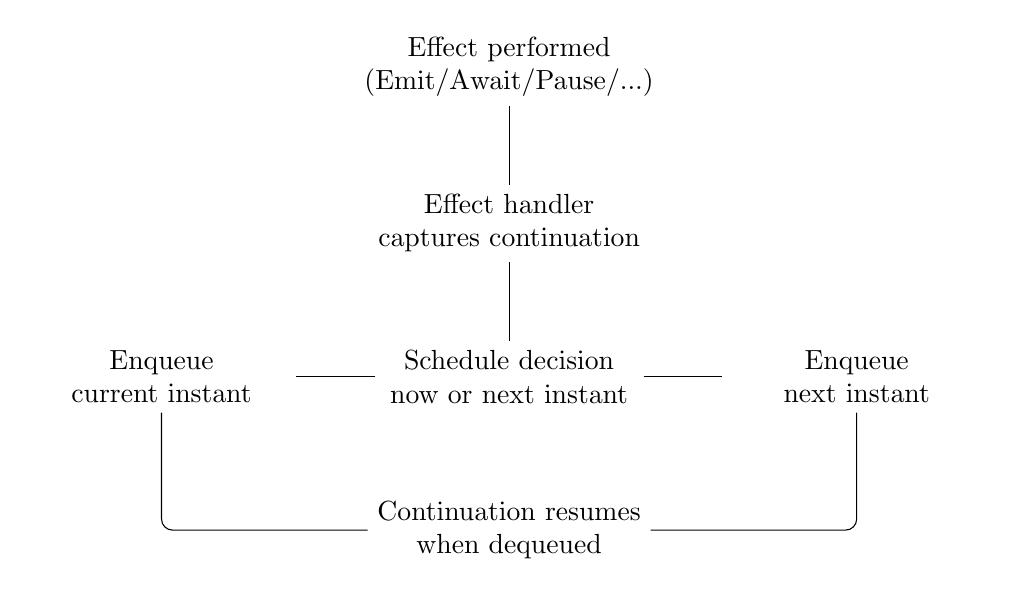
\begin{tikzpicture}[
  node distance=10mm,
  box/.style=tempo,
  draw,
  rounded corners,
  align=center,
  minimum width=34mm,
  minimum height=8mm,
  arrow/.style=tempo
]
\node[box] (effect) {Effect performed\\(Emit/Await/Pause/...)};
\node[box, below=of effect] (handler) {Effect handler\\captures continuation};
\node[box, below=of handler] (decision) {Schedule decision\\now or next instant};
\node[box, left=of decision] (now) {Enqueue\\current instant};
\node[box, right=of decision] (next) {Enqueue\\next instant};
\node[box, below=of decision] (resume) {Continuation resumes\\when dequeued};

\draw[arrow] (effect) -- (handler);
\draw[arrow] (handler) -- (decision);
\draw[arrow] (decision) -- (now);
\draw[arrow] (decision) -- (next);
\draw[arrow] (now) |- (resume);
\draw[arrow] (next) |- (resume);
\end{tikzpicture}%
}
\caption{Effect handling and continuation scheduling.}
\end{figure}

In the next section, we show how \tempo{} uses these mechanisms to implement a
synchronous runtime with explicit instants, signals, and control primitives.

\section{Implementation with Algebraic Effects (OCaml 5.3)}
This section can be read independently; it connects the public API to the
runtime mechanisms and effect handlers.
\tempo{} implements its synchronous model as a handler-driven runtime. The design
keeps the semantics explicit in library code while using OCaml 5.3 algebraic
effects to capture and schedule continuations. This section focuses on how the
effects-based implementation realizes the \tempo{} API.

\paragraph{Implementation map}
For readers skimming the code, the implementation can be read in three passes:
(1) the effect declarations in \texttt{lib/tempo\_types.ml}; (2) the scheduler
loop and task queues in \texttt{lib/tempo.ml}; (3) the handlers for each effect
in the same file. The most important invariant to keep in mind is that all
continuations are resumed by enqueueing tasks, never by direct calls, which
preserves the instant discipline.

\paragraph{Scheduler state and task queues}
The runtime maintains three task collections: a FIFO queue of tasks runnable
in the current instant, a list of tasks scheduled for the next instant, and a
list of tasks blocked on unsatisfied guards. Each task carries its guards and
preemption tokens, and tasks are grouped into logical threads so that
\texttt{join} can synchronize on thread completion. A registry of signals
tracks presence, current value, and waiting continuations.

The scheduler state also stores debug counters (signal ids, task ids, step and
instant counters) and a per-thread bookkeeping table. Each thread state keeps
an active task count and a list of waiters to resume when the thread completes.
This enables \texttt{join} to synchronize without global locks or OS threads.

The scheduler is single-threaded and deterministic: all decisions are made in
one runtime loop. This makes it easier to reason about the ordering of effects
within an instant, but it also means that the implementation must explicitly
track every deferred continuation to avoid hidden control flow.

Tasks move between queues as follows: when a task performs an effect that
defers it (e.g., \texttt{await} or \texttt{pause}), its continuation is wrapped
as a new task and enqueued in \texttt{next\_instant}. When a task is blocked by
guards, it is placed in the \texttt{blocked} list and also registered in the
missing signals' \texttt{guard\_waiters}. At instant end, all blocked tasks are
moved to \texttt{next\_instant}, preserving the rule that absent guards only
become observable in the next instant.

The scheduler also maintains a clear quiescence condition: an instant ends
only when the current queue is empty. This ensures that all reactions to
present signals have been taken before finalization, aligning with the
delayed-absence semantics.

\paragraph{Task lifecycle and bookkeeping}
Creating a task registers it under a thread id and increments the active count.
When a task finishes, the active count is decremented; if it reaches zero, any
waiters are resumed. Tasks carry a \emph{queued} flag to avoid double enqueue,
a \emph{blocked} flag to control guard rescheduling, and a list of kill tokens
that determine whether the task is still alive. This lifecycle is essential to
the deterministic semantics because it ensures tasks are resumed only at
well-defined instant boundaries.

\paragraph{Threads, \texttt{fork}, and \texttt{join}}
A \texttt{fork} creates a new logical thread with its own task counter. The
parent task continues immediately, while the child task is scheduled in the
current instant. \texttt{join} captures the caller's continuation and registers
it in the target thread's waiter list. When the thread's active counter reaches
zero, all join waiters are resumed in the next instant. This design allows
structured concurrency without OS threads, while still making completion
observable at instant boundaries.

\begin{lstlisting}[style=tempo]
(* Pseudo-code for join handling *)
on Join thread_id:
  if thread completed then
    enqueue_next (continue k ())
  else
    add waiter (fun () -> enqueue_next (continue k ()))
\end{lstlisting}

\paragraph{Invariants}
The scheduler maintains several invariants that are critical for correct
behavior:
\begin{itemize}
\item \textbf{No direct resumption}: every continuation becomes a task and is
  enqueued through the scheduler queues.
\item \textbf{No re-entrancy}: a task is never scheduled while it is already
  running (\texttt{queued} flag).
\item \textbf{Guard discipline}: a blocked task appears in guard\_waiters of
  every missing guard and nowhere else.
\item \textbf{Kill discipline}: a task is scheduled only if all its kill tokens
  are alive.
\end{itemize}
Most of the implementation complexity exists to preserve these invariants in
the presence of nested guards, nested preemption, and parallel composition.

\paragraph{Failure modes and debug hooks}
Several runtime checks enforce the synchronous discipline:
\begin{itemize}
\item \textbf{Multiple emits on event signals}: a second emission in the same
  instant raises an exception because the event semantics require a single
  value per instant.
\item \textbf{Present-without-value}: if a signal is marked present but has no
  stored value, the runtime fails fast to avoid undefined behavior.
\item \textbf{Dead kill tokens}: tasks protected by aborted kill tokens are
  discarded silently; this is intentional and implements weak preemption.
\end{itemize}
Debug counters (task ids, signal ids, instant/step counters) and optional logs
make it possible to correlate observable outputs with internal queue states.
These hooks are crucial when diagnosing unexpected blocking or when confirming
that a program respects the instant discipline.

\paragraph{Core runtime types}
The implementation centers on a small set of runtime records. The following
summary aligns with the concrete types in \texttt{lib/tempo\_types.ml} and
\texttt{lib/tempo.ml}.
\begin{table}[h]
\centering
\begin{tabularx}{\linewidth}{lY}
\hline
Type & Role and fields (informal) \\ \hline
\texttt{task} & \texttt{t\_id}, \texttt{thread}, \texttt{guards}, \texttt{kills},
\texttt{run}, plus \texttt{queued}/\texttt{blocked} flags. \\
\texttt{signal\_core} & \texttt{s\_id}, \texttt{present}, \texttt{value},
\texttt{awaiters}, \texttt{guard\_waiters}, and \texttt{kind} (event or
aggregate with \texttt{combine}/\texttt{initial}). \\
\texttt{thread\_state} & \texttt{active}, \texttt{completed}, \texttt{waiters}. \\
\texttt{scheduler\_state} & \texttt{current}, \texttt{next\_instant},
\texttt{blocked}, \texttt{signals}, \texttt{thread\_counter}, \texttt{threads},
and \texttt{debug} counters. \\ \hline
\end{tabularx}
\caption{Key runtime structures used by the scheduler.}
\end{table}

\paragraph{Declared effects}
The reactive operations are exposed as algebraic effects in
\texttt{lib/tempo\_types.ml}. The code below mirrors the actual declaration:
\begin{lstlisting}[style=tempo]
type _ Effect.t +=
  | New_signal : unit -> ('a, 'a, event) signal_core Effect.t
  | New_signal_agg :
      'agg * ('agg -> 'emit -> 'agg)
      -> ('emit, 'agg, aggregate) signal_core Effect.t
  | Emit : ('emit, 'agg, 'mode) signal_core * 'emit -> unit Effect.t
  | Await : ('emit, 'agg, 'mode) signal_core -> 'agg Effect.t
  | Await_immediate : ('a, 'a, event) signal_core -> 'a Effect.t
  | Pause : unit Effect.t
  | Fork : (unit -> unit) -> thread Effect.t
  | Join : thread -> unit Effect.t
  | With_guard :
      ('emit, 'agg, 'mode) signal_core * (unit -> unit) -> unit Effect.t
  | With_kill : kill * (unit -> unit) -> unit Effect.t
\end{lstlisting}
Each effect corresponds to a single scheduler action: \texttt{New\_signal}
allocates a fresh signal; \texttt{Emit} publishes a value and wakes waiters;
\texttt{Await}/\texttt{Await\_immediate} suspend and resume continuations;
\texttt{Pause} shifts execution to the next instant; \texttt{Fork}/\texttt{Join}
manage logical threads; and \texttt{With\_guard}/\texttt{With\_kill} implement
guarding and weak preemption.

\paragraph{From effect to scheduler (worked example)}
Consider \texttt{Await} as implemented in \texttt{lib/tempo.ml}. When a task
performs \texttt{Await s}, the handler captures the continuation and registers
it in \texttt{s.awaiters}. If \texttt{s} is already present and is an event
signal, the continuation is scheduled for the next instant; otherwise it is
stored as a waiter and resumed when \texttt{s} becomes present. The critical
behavior is that resumption is \emph{always} scheduled through the scheduler
queue, never executed directly in the current stack, which preserves the
instant boundary discipline.

In the excerpt below, the helper \texttt{mk\_task} wraps a continuation into a
runnable task. \texttt{enqueue\_next} schedules it for the next instant, and
\texttt{continue k v} resumes the captured continuation with value \texttt{v}.

\begin{lstlisting}[style=tempo]
(* lib/tempo.ml: effect handling for Await *)
| effect (Await s), k ->
    let enqueue_resume v =
      let t' = mk_task st t.thread t.guards t.kills
        (fun () -> continue k v) in
      enqueue_next st t'
    in
    let register_waiter () =
      let resume v =
        let t' = mk_task st t.thread t.guards t.kills
          (fun () -> continue k v) in
        enqueue_next st t'
      in
      s.awaiters <- resume :: s.awaiters
    in
    if s.present then
      match s.kind with
      | Event_signal ->
          (match s.value with
           | Some v -> enqueue_resume v
           | None -> failwith "present but no value")
      | Aggregate_signal _ ->
          register_waiter ()
    else
      register_waiter ()
\end{lstlisting}

In terms of observable behavior, this means that an \texttt{await} never
resumes in the current instant; the continuation is always deferred to the
next instant, ensuring that presence and absence are observed only at instant
boundaries. This pattern is representative of how effects encode the scheduler
policy in user space.

\begin{table}[h]
\centering
\begin{tabularx}{\linewidth}{lY}
\hline
Effect & Scheduler action and instant semantics \\ \hline
\texttt{New\_signal} & Allocate signal state in the current instant. \\
\texttt{Emit} & Mark present and wake awaiters (possibly now). \\
\texttt{Await} & Register continuation; resume next instant. \\
\texttt{Await\_immediate} & Resume now if present; otherwise register waiter. \\
\texttt{Pause} & Defer continuation to the next instant. \\
\texttt{Fork} & Spawn child task in current instant. \\
\texttt{Join} & Suspend until thread completes, then resume. \\
\texttt{With\_guard} & Attach guard set; block if guards absent. \\
\texttt{With\_kill} & Register cleanup; abort at instant end on kill. \\ \hline
\end{tabularx}
\caption{Effect-to-scheduler mapping.}
\end{table}

\paragraph{Instant loop and signal finalization}
Execution proceeds by instants. During an instant, the scheduler repeatedly
dequeues a runnable task, checks whether its guards are satisfied, and either
runs it or moves it to the blocked list. At the end of the instant, the
runtime finalizes all signals: event and aggregate signals are reset to
absent, guard waiters are cleared, and aggregate-signal awaiters are resumed
with the accumulated value. Blocked tasks are moved to the next-instant list,
and the next instant begins with the tasks that remain alive.

More precisely, each step records timing metrics, logs queue snapshots, and
updates counters for reproducibility. When the runnable queue becomes empty,
the instant ends. All blocked tasks are re-queued for the next instant, which
implements the delayed-absence discipline: a guard that was absent remains
absent for the entire instant, and the task can only retry in the next one.

Re-queuing does not lose guard information: the blocked task still carries its
guard list, so when it is dequeued in the next instant it is checked again. If
some guards are still absent, it is re-registered in the corresponding
\texttt{guard\_waiters} lists. This is why clearing \texttt{guard\_waiters} at
instant end is safe: the lists are reconstructed as tasks are revisited.

\paragraph{Queue discipline and fairness}
The current queue is FIFO, which yields a simple notion of fairness within an
instant: tasks are resumed in the order they are enqueued. This ordering is an
implementation choice rather than a semantic guarantee, and observable results
should not depend on it. The ordering is nevertheless useful for debugging and
reproducible traces, and it aligns with the cooperative scheduling model of
FairThreads.

To avoid starvation across instants, any task that remains blocked is
reconsidered in the next instant. This provides a coarse-grained fairness
property: if a guard becomes present in some future instant, the corresponding
task will be eligible to run at the start of that instant.

\paragraph{Instant loop pseudo-code}
\begin{lstlisting}[style=tempo]
while current_queue not empty do
  t <- pop current_queue
  if not kills_alive t then discard t
  else if guard_ok t.guards then run t
  else
    block t on missing_guards
    register t in guard_waiters of each missing guard
end
finalize_signals ()
move blocked tasks to next_instant
swap current_queue and next_instant
\end{lstlisting}
This sketch omits bookkeeping details (thread counters, debug logs) but
captures the control structure of the scheduler.

The ordering above is deliberate. Kill checks precede guard checks so that a
preempted task is never allowed to run or block again. Guard checks precede
execution to preserve the semantics that guards are blocking conditions, not
filters applied after a step. If these checks were reversed, a task might run
in an instant where its guard is absent or continue after being preempted,
which would violate the intended weak-preemption semantics.

\begin{figure}[t]
\centering
\resizebox{0.80\columnwidth}{!}{%
\footnotesize
\begin{tikzpicture}[
  node distance=10mm,
  box/.style=tempo,
  draw,
  rounded corners,
  align=center,
  minimum width=30mm,
  minimum height=8mm,
  decision/.style=tempo,
  draw,
  align=center,
  aspect=2,
  inner sep=1pt,
  arrow/.style=tempo
]
\node[box] (start) {Start instant};
\node[box, below=of start] (dequeue) {Dequeue task};
\node[decision, below=of dequeue] (guards) {Guards\\satisfied?};
\node[box, left=of guards] (block) {Block task\\on guards};
\node[box, right=of guards] (handle) {Handle task\\effects};
\node[decision, below=of guards] (empty) {Queue\\empty?};
\node[box, below=of empty] (finalize) {Finalize signals\\and move blocked};
\node[box, below=of finalize] (next) {Next instant};

\draw[arrow] (start) -- (dequeue);
\draw[arrow] (dequeue) -- (guards);
\draw[arrow] (guards) -- node[above]{no} (block);
\draw[arrow] (guards) -- node[above]{yes} (handle);
\draw[arrow] (block) |- (empty);
\draw[arrow] (handle) |- (empty);
\draw[arrow] (empty) -- node[right]{yes} (finalize);
\draw[arrow] (empty) -- ++(20mm,0mm) node[right]{no} |- (dequeue);
\draw[arrow] (finalize) -- (next);
\end{tikzpicture}%
}
\caption{High-level flowchart of the instant-based scheduler.}
\end{figure}

\paragraph{Execution trace (guard + watch)}
Consider the running example from Section~\ref{ex:guard-watch}. In instant $t$,
one task is guarded by signal \texttt{g}, and one is wrapped in \texttt{watch s}.
At the start of the instant, both tasks are in the current queue. The guarded
task is blocked because \texttt{g} is absent and is registered in
\texttt{g.guard\_waiters}. The watched task runs; if it emits \texttt{s} during
$t$, the guardian aborts the kill token and the watched task is prevented from
continuing into $t{+}1$. At instant end, guard waiters are cleared, blocked
tasks are moved to the next-instant list, and the system advances. This trace
illustrates how guard blocking and weak preemption interact with the instant
boundary discipline.

\begin{lstlisting}[style=tempo]
let g = new_signal () in
let s = new_signal () in
let guarded = (fun () -> when_ g (fun () -> emit s ())) in
let watched = (fun () -> watch s (fun () -> pause (); emit s ())) in
parallel [guarded; watched]
\end{lstlisting}
The trace tables below show the corresponding queue, signal, and observable
states across instants.

\begin{table}[h]
\centering
\begin{tabularx}{\linewidth}{lY}
\hline
Instant & Queue/blocked/signals snapshot \\ \hline
$t$ start & Current: \texttt{guarded}, \texttt{watched}; blocked: $\varnothing$;
signals: $g=\bot$, $s=\bot$. \\
$t$ mid & \texttt{guarded} blocked on $g$; \texttt{watched} runs and emits $s=()$;
kill token marked. \\
$t$ end & Guard waiters cleared; blocked $o$ next instant; $s$ observed
present at boundary, then reset; \texttt{watched} will not continue into
$t{+}1$. \\ \hline
\end{tabularx}
\caption{Concrete execution trace for guard + watch (example above).}
\end{table}

\begin{table}[h]
\centering
\begin{tabularx}{\linewidth}{lY}
\hline
Instant & Observable signals and outputs \\ \hline
$t$ & $s=()$ becomes present due to \texttt{watched}; no output emitted. \\
$t{+}1$ & \texttt{guarded} remains blocked if $g=\bot$; no output emitted. \\
\hline
\end{tabularx}
\caption{Two-instant observable trace for the example program.}
\end{table}

\paragraph{Signal operations}
Signal creation effects allocate runtime state and register signals in the
global registry. \texttt{Emit} marks a signal present and stores its value.
For event signals, multiple emissions in the same instant are rejected, while
aggregate signals fold successive emissions into an accumulator. Awaiting a
signal registers a continuation: \texttt{await} always resumes at the next
instant, while \texttt{await\_immediate} can resume in the current instant when
the event signal is already present. This distinction matches the delayed
absence discipline while still allowing immediate reactions when safe.
Figure~\ref{fig:signal-state} summarizes the signal state evolution within a
single instant.

Event signals enforce a single-emission rule. The implementation checks
\texttt{s.present} and raises an exception on a second emission in the same
instant. This runtime check enforces the synchronous discipline in the absence
of static typing rules.

Signal waiters are stored as callbacks (continuations wrapped as functions).
For event signals, each emission registers resumption through the scheduler;
\texttt{await} resumes in the next instant, while \texttt{await\_immediate} may
resume in the current instant if the signal is already present. For aggregate
signals, emissions only update the accumulator; awaiters are resumed once at
instant end with the aggregated value. This makes the point of observation
explicit and keeps the aggregation order-insensitive.

Aggregate signals are delivered only once per instant. Emissions update the
accumulator, but awaiters are resumed at instant end with the accumulated
value. This preserves determinism because the order of emissions within the
instant does not affect the observable schedule, only the aggregated result.
If the combine function is not associative/commutative, the aggregate value may
still depend on intra-instant evaluation order, which is intentionally left
unspecified; this is why the API recommends pure, order-insensitive combines.

The finalization step can be summarized as follows:
\begin{lstlisting}[style=tempo]
for each signal s in registry do
  if s is aggregate then
    resume all awaiters with s.value
  clear s.awaiters and s.guard_waiters
  reset s.present and s.value
\end{lstlisting}
In the actual implementation, event-signal awaiters have already been resumed
on emission, whereas aggregate awaiters are resumed in this finalization phase.

\begin{figure}[t]
\centering
\resizebox{0.92\columnwidth}{!}{%
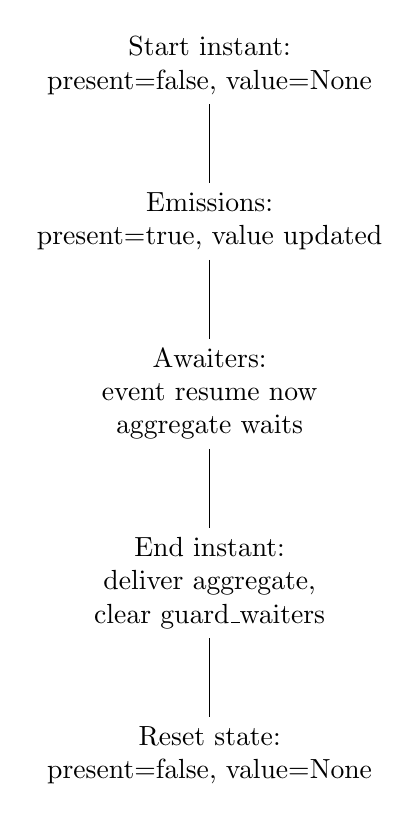
\begin{tikzpicture}[
  node distance=10mm,
  box/.style=tempo,
  draw,
  rounded corners,
  align=center,
  minimum width=36mm,
  minimum height=8mm,
  arrow/.style=tempo
]
\node[box] (start) {Start instant:\\present=false, value=None};
\node[box, below=of start] (emit) {Emissions:\\present=true, value updated};
\node[box, below=of emit] (awaiters) {Awaiters:\\event resume now\\aggregate waits};
\node[box, below=of awaiters] (finalize) {End instant:\\deliver aggregate,\\clear guard\_waiters};
\node[box, below=of finalize] (reset) {Reset state:\\present=false, value=None};

\draw[arrow] (start) -- (emit);
\draw[arrow] (emit) -- (awaiters);
\draw[arrow] (awaiters) -- (finalize);
\draw[arrow] (finalize) -- (reset);
\end{tikzpicture}%
}
\caption{Signal state evolution within an instant.}
\label{fig:signal-state}
\end{figure}

\paragraph{Guards and blocking}
Guarded execution is implemented by attaching a list of guard signals to each
task. If a guard is missing, the task is blocked and registered in the guard
waiter lists of the missing signals. When a signal is emitted, its guard
waiters are rechecked: tasks whose guards are now all present are moved back to
the runnable queue, otherwise they remain blocked on the remaining missing
guards. This implements the disjunctive behavior of nested guards while
preserving determinism.

Guard checking is centralized: \texttt{guard\_ok} verifies all guards are
present, while \texttt{missing\_guards} returns the absent subset. This keeps
guard logic explicit and ensures the scheduler, rather than user code, controls
when a blocked task can resume.

To avoid repeated scans, each signal maintains its own \texttt{guard\_waiters}
list. When a signal becomes present, only tasks that were blocked on that
signal are reconsidered. Tasks may remain blocked if other guards are still
absent, and they are re-registered on the remaining missing guards. This local
indexing keeps guard rescheduling proportional to the number of blocked tasks
that are directly affected by the emission.

\paragraph{Guard disjunction by nesting}
Nested \texttt{when\_} expressions behave as a conjunction at the level of
guard satisfaction: a task blocked on multiple guards remains blocked until
\emph{all} guards are present in the same instant. If a program wants a logical
disjunction (guard $g_1$ \emph{or} $g_2$), it must use parallel guarded
branches, which creates distinct tasks each blocked on a single guard. This
mechanism follows directly from the guard list representation and the
centralized \texttt{guard\_ok} predicate.

\paragraph{Effect \texttt{With\_guard} and \texttt{when\_}}
The \texttt{when\_} combinator is implemented using the \texttt{With\_guard}
effect. Performing \texttt{With\_guard (s, body)} creates a new task whose
guard list is extended with \texttt{s}. If \texttt{s} is absent, the task is
blocked and registered in \texttt{s.guard\_waiters}. Once \texttt{s} becomes
present, the scheduler rechecks the guard list and enqueues the task in the
current instant. This means that \texttt{when\_} does not execute \texttt{body}
until the guard is satisfied, and the scheduling decision remains centralized.
In the excerpt below, \texttt{Any s} wraps a typed signal into an existential
for the guard list, and \texttt{enqueue\_now} schedules the guarded task in the
current instant.
\begin{lstlisting}[style=tempo]
(* lib/tempo.ml: effect handling for With_guard *)
| effect (With_guard (s, body)), k ->
    let t' =
      mk_task st t.thread (Any s :: t.guards) t.kills
        (fun () ->
          body ();
          enqueue_now st (mk_task st t.thread t.guards t.kills
            (fun () -> continue k ())))
    in
    enqueue_now st t'
\end{lstlisting}

\paragraph{Guard resumption trace}
Consider a task guarded by $g_1$ and $g_2$. At instant $t$, $g_1$ is present
but $g_2$ is absent. The task is blocked and registered in $g_2.guard\_waiters$
only; it is not re-checked until $g_2$ becomes present. When $g_2$ is emitted
in instant $t{+}1$, the scheduler revisits the task, finds all guards present,
and enqueues it in the current queue. This preserves the intended "all guards
in the same instant" semantics.

\paragraph{Effect \texttt{With\_kill} and \texttt{watch}}
Weak preemption relies on the \texttt{With\_kill} effect. A kill token stores a
cleanup continuation that is invoked when the token is aborted. The \texttt{watch}
combinator creates a shared kill token for the protected body and a guardian
task that waits on the watched signal. When the signal is emitted, the guardian
aborts the shared token, which triggers the cleanup and prevents further
resumption of the protected task.

Concretely, \texttt{watch} runs the body under \texttt{With\_kill} and installs
a cleanup continuation that schedules the parent continuation at the appropriate
instant boundary. The scheduler checks \texttt{kills\_alive} before enqueuing a
task, so any task protected by an aborted kill token is discarded. This yields
weak preemption: the body can finish the current instant, but it will not
continue in subsequent instants once the watched signal is present.
In the excerpt below, \texttt{continue\_now} resumes the parent continuation in
the current instant, while \texttt{continue\_later} defers it to the next
instant. The cleanup stored in \texttt{kk.cleanup} chooses the safe resumption
point once the kill token is aborted.
\begin{lstlisting}[style=tempo]
(* lib/tempo.ml: effect handling for With_kill *)
| effect (With_kill (kk, body)), k ->
    let continue_now () =
      kk.cleanup <- None;
      enqueue_now st (mk_task st t.thread t.guards t.kills
        (fun () -> continue k ()))
    and continue_later () =
      kk.cleanup <- None;
      enqueue_next st (mk_task st t.thread t.guards t.kills
        (fun () -> continue k ()))
    in
    kk.cleanup <- Some continue_later;
    let runner () =
      body ();
      continue_now ()
    in
    let t' = mk_task st t.thread t.guards (kk :: t.kills) runner in
    enqueue_now st t'
\end{lstlisting}

\paragraph{Worked walkthrough: \texttt{watch}}
Consider a body \texttt{B} under \texttt{watch s}. At instant $t$, the guardian
awaits \texttt{s} while \texttt{B} runs. If \texttt{s} is emitted during $t$,
the guardian aborts the shared kill token and installs cleanup to prevent
\texttt{B} from continuing at $t{+}1$. If \texttt{s} is not emitted, \texttt{B}
continues normally in the next instant. This aligns with weak preemption: the
body can complete the current instant but is cut off before the next one.

\paragraph{Weak preemption with kill tokens}
Weak preemption is modeled through kill tokens. A \texttt{watch} spawns a
guardian that waits on the watched signal and aborts the protected computation
at the end of the instant in which the signal is emitted. Internally, the
runtime stores cleanup continuations for kill tokens so that aborting a token
can schedule the appropriate continuation either immediately or in the next
instant. This approach encodes preemption without violating the single-instant
deterministic semantics.

Kill tokens also ensure that tasks are not resumed after preemption. The
scheduler checks that all kill tokens are alive before enqueuing a task; if any
token is dead, the task is discarded and the thread bookkeeping is updated.
Because preemption is weak, application code sometimes adds an explicit guard
(e.g., a \texttt{handled} signal) to prevent simultaneous emissions in the same
instant; this pattern is illustrated in the usage examples.

\paragraph{Kill tokens and nested \texttt{watch}}
Nested \texttt{watch} constructs install multiple kill tokens. The scheduler
checks that \emph{all} kill tokens are alive before running a task. This means
any inner \texttt{watch} that aborts its token is sufficient to prevent the
task from continuing, which realizes the intended disjunction of stopping
conditions. Kill tokens do not cancel the current instant; they only prevent
the continuation from being enqueued after the instant boundary, which
preserves weak preemption.

\paragraph{Kill cleanup timing}
The cleanup stored in a kill token is intentionally deferred with respect to
observable behavior: if the watched signal is emitted in instant $t$, the
protected computation can still finish its current instant but will not be
resumed in $t{+}1$. Internally, the handler may schedule the cleanup either
immediately or for the next instant, but the user-visible effect is always
weak preemption at the instant boundary.

\paragraph{Host I/O hooks}
The entry point \texttt{execute} creates dedicated input and output signals.
Before each step, host input can emit on the input signal; after the step, the
output signal is checked and delivered to the host. This keeps external I/O
separate from synchronous reactions while preserving the instant structure.

Internally, \texttt{execute} installs a handler for all effects and runs a
driver loop that alternates between (1) injecting host input for the instant,
(2) running the scheduler until quiescence, and (3) collecting the output
signal. This design keeps the host side free of continuation manipulation: the
host only sees a stream of inputs and outputs at instant boundaries, which is
consistent with the synchronous model.

\begin{lstlisting}[style=tempo]
loop:
  call input_hook to emit on input signal
  run scheduler until current queue is empty
  read output signal at instant end
\end{lstlisting}
Outputs are therefore observed only at instant boundaries, which matches the
delayed-absence discipline and prevents mid-instant I/O from leaking
implementation order.

For readability, helper functions used in the excerpts are summarized below
(see Section~\ref{sec:helper-glossary}).

\paragraph{Runtime helper glossary}\label{sec:helper-glossary}
\begin{itemize}
\item \texttt{mk\_task}: wrap a continuation into a runnable task record.
\item \texttt{enqueue\_now}: schedule a task in the current instant queue.
\item \texttt{enqueue\_next}: schedule a task for the next instant.
\item \texttt{continue}: resume a captured continuation with a value.
\item \texttt{Any}: existential wrapper to store signals in guard lists.
\item \texttt{kills\_alive}: check that all kill tokens of a task are alive.
\end{itemize}

\subsection{Algebraic Effects in Detail}
	\tempo{} encodes the reactive primitives as algebraic effects and interprets them
with a deep handler. Each effect represents a semantic action (e.g., emit,
await, pause), and the handler decides whether to resume the continuation now
or to re-schedule it for a later instant. This design makes the control flow
explicit and keeps the scheduler in user space rather than in a custom runtime.

Effect capture preserves the current continuation, which is then wrapped into a
task structure. For example, \texttt{await} captures the continuation, stores a
resume function in the signal's waiter list, and ensures that the continuation
is resumed at the beginning of the next instant. \texttt{await\_immediate}
selects between immediate resumption (if the signal is already present) and
registration as a waiter (if it is not). Similarly, \texttt{pause} captures the
continuation and places it in the next-instant list.

Signal creation effects allocate fresh signal records and return them to the
continuation. \texttt{Emit} updates signal state and resumes any registered
awaiters, potentially in the current instant. Guard effects update the task's
guard set and may block the task if the guards are not satisfied. Preemption
effects (\texttt{With\_kill}) store cleanup continuations that are invoked when
the kill token is aborted, ensuring that termination is coordinated with the
instant boundary.

This effect-based organization provides a clear separation between the
operational model (captured by the handler) and the user-facing API (exposed as
effectful functions). It also enables experimentation with scheduling
strategies without changing the OCaml runtime or the language semantics.

\paragraph{Handler pseudo-code}
\begin{lstlisting}[style=tempo]
handle task =
  match task() with
  | effect (Emit (s, v)) k ->
      mark_present s v;
      resume_awaiters s;
      enqueue_now (continue k ())
  | effect (Await s) k ->
      register_waiter s (fun v -> enqueue_next (continue k v))
  | effect (Await_immediate s) k ->
      if present s then enqueue_now (continue k (value s))
      else register_waiter s (fun v -> enqueue_now (continue k v))
  | effect Pause k ->
      enqueue_next (continue k ())
  | effect (With_guard (s, body)) k ->
      update_guards s;
      enqueue_now (fun () -> body (); continue k ())
  | effect (With_kill (kk, body)) k ->
      install_cleanup kk (fun () -> enqueue_next (continue k ()));
      enqueue_now (fun () -> body (); continue k ())
  | effect (Fork f) k ->
      enqueue_now f; enqueue_now (continue k ())
  | effect (Join t) k ->
      add_join_waiter t (fun () -> enqueue_now (continue k ()))
\end{lstlisting}

\subsection{Detailed Effect Traces}
This subsection provides step-by-step traces for key primitives. The goal is
to make explicit where continuations are stored and how they move across
queues.

\paragraph{Trace: \texttt{await\_immediate}}
Suppose \texttt{s} is an event signal. If \texttt{s} is already present, the
continuation is resumed in the current instant via \texttt{enqueue\_now};
otherwise it is registered in \texttt{s.awaiters} for resumption at the next
instant. The behavior is summarized below.
\begin{table}[h]
\centering
\begin{tabularx}{\linewidth}{lY}
\hline
Case & Scheduler action \\ \hline
\texttt{s.present=true} & Enqueue continuation now; current instant resumes. \\
\texttt{s.present=false} & Store waiter; resume at next instant. \\ \hline
\end{tabularx}
\caption{Scheduler actions for \texttt{await\_immediate}.}
\end{table}

\paragraph{Trace: \texttt{pause}}
\texttt{pause} captures the current continuation and enqueues it for the next
instant. The task does not run again in the current instant, which is the
primary mechanism for separating instants in user code.

\paragraph{Trace: \texttt{parallel}}
\texttt{parallel} spawns multiple tasks in the current instant and waits for
their completion. It relies on \texttt{fork} under the hood: each branch is a
child task, and the parent waits until the child thread's active count reaches
zero. The effect-level view is therefore:
\begin{enumerate}
\item Spawn a child task for each branch.
\item Continue parent task to a \texttt{join}-like waiting point.
\item Resume parent once all branches terminate.
\end{enumerate}

\paragraph{Trace: \texttt{watch}}
The following sketch shows the lifecycle of a watched task.
\begin{table}[h]
\centering
\begin{tabularx}{\linewidth}{lY}
\hline
Step & Scheduler action \\ \hline
Start $t$ & Spawn guardian awaiting $s$; run body task. \\
$s$ emitted & Guardian aborts kill token; installs cleanup. \\
End $t$ & Body may complete; continuation not enqueued for $t{+}1$. \\
$t{+}1$ & Body is discarded if kill token is dead. \\ \hline
\end{tabularx}
\caption{Execution trace for \texttt{watch}.}
\end{table}

\paragraph{Trace: \texttt{when\_}}
The guard handler creates a task with an extended guard list. If the guard is
absent, the task is blocked; if the guard is present, the task is enqueued
immediately. The observable result is that \texttt{body} only begins in an
instant where the guard is present.

\subsection{Code Map: from API to Runtime}
The table below provides a roadmap from surface-level functions to the runtime
mechanisms that implement them. This can be used as a guide when reading the
source.
\begin{table}[h]
\centering
\begin{tabularx}{\linewidth}{lY}
\hline
API function & Runtime mechanism \\ \hline
\texttt{new\_signal} & \texttt{New\_signal} effect, allocates signal\_core. \\
\texttt{new\_signal\_agg} & \texttt{New\_signal\_agg} effect, sets combine/init. \\
\texttt{emit} & \texttt{Emit} effect, updates signal and wakes waiters. \\
\texttt{await} & \texttt{Await} effect, registers waiter for next instant. \\
\texttt{await\_immediate} & \texttt{Await\_immediate} effect, immediate or next. \\
\texttt{pause} & \texttt{Pause} effect, enqueue for next instant. \\
\texttt{when\_} & \texttt{With\_guard} effect, extend guard list. \\
\texttt{watch} & \texttt{With\_kill} effect, install kill token/cleanup. \\
\texttt{parallel} & \texttt{fork}/\texttt{join}, thread counters. \\
\texttt{execute} & Scheduler loop + host I/O hooks. \\ \hline
\end{tabularx}
\caption{Mapping from API to runtime mechanisms.}
\end{table}

\section{Performance}
This section provides expected complexity and performance considerations in the
absence of dedicated benchmarks.

\paragraph{Scheduler complexity}
Let $T$ be the number of runnable tasks in an instant, $B$ the number of
blocked tasks, and $S$ the number of registered signals. The scheduler processes
each runnable task at most once per step and checks guard satisfaction by
scanning the task's guard list. Over an instant, the total cost is
$O(T + G)$ where $G$ is the sum of guard-list sizes across tasks, plus
signal finalization at $O(S)$.

\paragraph{Signal operations}
Emitting an event signal resumes all its awaiters immediately (in scheduler
terms), so the cost is proportional to the number of waiters on that signal.
Aggregate signals defer resumption to instant end, so emission cost is $O(1)$
plus the cost of the user-provided combine function. Finalization resumes all
aggregate awaiters once per instant.

\paragraph{Queue sizes and memory}
Memory usage grows with the number of tasks, signals, and registered waiters.
In typical use, each \texttt{await} adds one continuation to a signal's waiter
list, and each guard adds a task to a guard\_waiter list. Worst-case memory
consumption is therefore linear in the number of suspended tasks and guards.

\paragraph{Assumptions}
These bounds assume: (1) guard lists are short; (2) signals are not created at
unbounded rates per instant; (3) the combine function for aggregate signals is
constant-time. Under these assumptions, the scheduler is expected to scale
linearly with the number of active tasks and signals per instant.

\paragraph{Effect and allocation overhead}
Each reactive primitive is implemented as an effect, which captures a
continuation and allocates a task record. The dominant overheads are therefore
continuation capture, task allocation, and queue operations. In practice, this
means performance is sensitive to allocation rates and GC behavior, especially
in programs that spawn many short-lived tasks per instant.

\paragraph{Preemption and guard costs}
Weak preemption introduces a small constant overhead per protected task: a kill
token, a cleanup closure, and a liveness check when the task is enqueued. Guard
checks scale with the number of guard conditions attached to a task, which
makes guard-heavy programs more sensitive to the size of guard lists than to
the number of signals overall.

\paragraph{ReactiveML comparison plan}
To compare \tempo{} against ReactiveML, we propose a small benchmark suite that
captures the common synchronous patterns shared by both systems:
\begin{itemize}
\item \textbf{Ping-pong signals}: two processes alternately emit and await
  signals across instants (measures basic signaling and scheduling overhead).
\item \textbf{Barrier synchronization}: $N$ parallel tasks emit on a barrier
  signal and a coordinator waits for all emissions (measures aggregation and
  guard wakeups).
\item \textbf{Timeout and preemption}: a request handler guarded by a timeout,
  implemented with weak preemption (measures watch/guard overhead).
\item \textbf{Broadcast and fan-out}: one emitter wakes $N$ awaiters in the same
  instant (measures awaiter resumption cost).
\item \textbf{Guarded loops}: repeated guarded activation with pauses across
  many instants (measures long-running scheduling stability).
\end{itemize}
For each scenario, the metrics of interest are throughput (instants per second),
latency per instant, and memory usage as a function of the number of tasks and
signals. These benchmarks are intended as future work; the current draft does
not include measured results.

\paragraph{Benchmark parameters}
\begin{table}[h]
\centering
\begin{tabularx}{\linewidth}{lY}
\hline
Benchmark & Parameters and cost drivers \\ \hline
Ping-pong & $I$ instants; cost dominated by signal wakeups. \\
Barrier   & $N$ tasks; cost dominated by guard wakeups and aggregation. \\
Timeout   & $I$ instants; cost dominated by watch/kill handling. \\
Broadcast & $N$ awaiters; cost dominated by awaiter resumption. \\
Guarded loop & $I$ instants; cost dominated by guard checks per instant. \\ \hline
\end{tabularx}
\caption{Benchmark parameters and expected cost drivers.}
\end{table}

\paragraph{Reproducibility outline}
Each scenario can be implemented as a standalone executable in
\texttt{tests/ok} (\tempo{}) and a corresponding ReactiveML program, compiled with
the ReactiveML toolchain. A minimal protocol should record: (1) number of
instants executed; (2) wall-clock time; (3) task/signal counts. This makes the
comparison transparent even before results are reported.

\paragraph{Concrete protocol}
For each scenario, fix a parameter grid (e.g., number of tasks $N \in
\{10, 10^2, 10^3\}$ and instants $I \in \{10^3, 10^4\}$), and run both \tempo{} and
ReactiveML implementations on the same machine with CPU frequency scaling
disabled. Measure wall-clock time for $I$ instants, record peak resident memory,
and log the number of signals and waiters. Report median over at least 5 runs.

\paragraph{Test coverage map}\label{sec:feature-tests}
The list below shows which \texttt{tests/ok} programs exercise each public
feature. This supports the claim that all features are covered by tests.
\begin{itemize}
\item \textbf{emit/await}:
  \texttt{emit\_once\_await\_one.ml} \\
  \texttt{emit\_once\_await\_many.ml}.
\item \textbf{await\_immediate}: \texttt{emit\_once\_await\_immediate.ml},
  \\ \texttt{when\_await\_imm\_same\_instant.ml},
  \\ \texttt{when\_await\_imm\_next\_instant.ml}.
\item \textbf{pause}: \texttt{pause.ml}.
\item \textbf{parallel}: \texttt{parallel.ml}, \texttt{when\_parallel.ml}.
\item \textbf{guards/when\_}: \texttt{when\_next\_instant.ml},
  \\ \texttt{when\_same\_instant.ml}, \texttt{when\_nested.ml},
  \\ \texttt{when\_complete.ml}.
\item \textbf{watch/weak preemption}: \texttt{watch\_complete.ml},
  \\ \texttt{watch\_nested.ml}, \texttt{watch\_killed.ml},
  \\ \texttt{watch\_when\_complete.ml}, \texttt{watch\_when\_killed.ml}.
\item \textbf{kill}: \texttt{with\_kill\_abort.ml}, \texttt{with\_kill\_inherit.ml}.
\item \textbf{aggregate signals}:
  \texttt{emit\_agg\_collect.ml} \\
  \texttt{emit\_agg\_sum.ml}.
\item \textbf{present\_then\_else}: \texttt{present\_then\_else.ml}.
\end{itemize}

\paragraph{Testing strategy (summary)}
Tests are organized by primitive (signals, guards, preemption) and by
composition patterns (parallel, nested guards, immediate awaits). Each test
has an expected output, enabling regression checks on observable behavior at
instant boundaries.

\section{Limitations and Trade-offs}
\tempo{} is designed as a lightweight library-level runtime. This choice comes
with several limitations that define the current scope:
\begin{itemize}
\item \textbf{No static guarantees.} Determinism and correct use of primitives
  (e.g., single emission on event signals) are enforced at runtime rather than
  by a type system or compiler checks.
\item \textbf{Runtime errors for misuse.} Multiple emissions on an event signal
  raise an exception; misuse must be caught by tests or careful discipline.
\item \textbf{Effects require OCaml 5.3.} The approach relies on algebraic
  effects and deep handlers, which are not available in earlier versions.
\item \textbf{Library-level scheduling only.} \tempo{} does not integrate with a
  language-level optimizer, so certain static analyses or compile-time
  optimizations (as in ReactiveML) are unavailable.
\item \textbf{Low-level API risks.} The \texttt{Tempo.Low\_level} module exposes
  primitives that can break high-level invariants if used incorrectly.
\item \textbf{Determinism vs evaluation order.} Reference-based communication
  can make behavior depend on evaluation order within an instant, which is not
  fixed by the semantics; mitigating this requires static analyses (see
  Section~\ref{sec:future-work}).
\item \textbf{Purity assumptions.} Aggregate signals assume order-insensitive
  combine functions; if combine is not associative/commutative, aggregate
  results may depend on intra-instant scheduling.
\item \textbf{Logical parallelism only.} Concurrency is logical and single-core;
  enabling physical parallelism would require additional determinism controls
  (see Section~\ref{sec:future-work}).
\item \textbf{Non-guaranteed behaviors.} Programs relying on shared mutable
  state across parallel tasks can observe different results even with identical
  inputs, because the intra-instant order is unspecified.
\end{itemize}

\section{Related Work}
\tempo{} is rooted in the reactive control lineage: Esterel, FairThreads, and
ReactiveML. It inherits Boussinot's delayed-absence discipline
\cite{esterel1992,fairthreads2003,reactiveml2005}. Relative to Esterel, \tempo{}
does not impose a static compilation discipline; instead it targets dynamic
behavior and library-level composition. Relative to FairThreads, \tempo{} provides
a typed OCaml API with higher-order combinators and valued signals.

Other synchronous languages in the same family include Lustre and Signal, which
take dataflow-oriented approaches to synchronous programming, and the broader
survey literature that situates these languages in a shared semantic landscape
\cite{lustre1991,signal1987,benveniste2003}. \tempo{} aligns with this lineage but
focuses on control primitives realized at library level rather than a dedicated
compiler.

Industrial synchronous formalisms have also shaped this landscape. Statecharts
provide a widely adopted visual model for reactive control
\cite{harel1987statecharts}, and SCADE offers a synchronous design and
validation environment for safety-critical embedded control software
\cite{berry2007scade}. These systems emphasize predictable control behavior and
tooling, whereas \tempo{} targets a lightweight, library-level embedding.

Closely related academic languages include Lucid Synchrone and Quartz, which
extend synchronous ideas with functional or model-based design perspectives
\cite{caspihamonpouzet2008lucid,schneider2017quartz}. These reinforce the
continuity between \tempo{} and earlier synchronous language research.

ReactiveML is the closest antecedent: it integrates reactive constructs into a
language extension with dedicated syntax and compilation support. \tempo{}, by
contrast, is a pure library that relies on OCaml 5.3 algebraic effects to
implement the same control primitives without modifying the compiler or the
runtime. This makes \tempo{} easier to integrate into existing OCaml codebases and
enables experimentation with scheduling policies in user space, at the cost of
foregoing some static analyses and language-level guarantees provided by
ReactiveML.

In contrast with FRP \cite{frp1997}, \tempo{} emphasizes control and instant-based
determinism rather than continuous dataflow. The library focuses on explicit
signals, guards, and preemption, aligning with synchronous reactive semantics
instead of stream processing abstractions.

Stream-processing languages such as Lucid and StreamIt
\cite{ashcroft1977lucid,thies2002streamit} emphasize dataflow pipelines rather
than control-centric instants. They provide a useful contrast to \tempo{}: the
dataflow style is oriented toward throughput and steady-state streaming, while
\tempo{} targets explicit control reactions at discrete instants.

Recent FRP systems have introduced stronger operational guarantees. The
modal FRP line of work uses modal types to enforce causality and prevent space
leaks, including Simply RaTT and its extensions
\cite{bahr2019ratt,bahr2022modalfrp,bahr2023async}. These systems target
dataflow FRP rather than control-oriented primitives, but they offer insights
into static enforcement mechanisms that could complement \tempo{}'s current
runtime checks.
Recent applications of modal FRP include GUI programming with modal types,
which demonstrates the practicality of these systems in reactive user
interfaces \cite{bahr2025gui}.

Industrial reactive-streams frameworks (e.g., RxJava, Akka Streams) emphasize
asynchronous stream processing and backpressure rather than synchronous
instants. While their semantics differ from \tempo{}'s model, they represent a
separate lineage of reactive programming practice and are surveyed in the
reactive-streams literature \cite{cheng2017reactivestreams,davis2019reactivestreams}.

\tempo{} also builds on the recent availability of algebraic effects and handlers
in OCaml \cite{multicoreocaml2020}. At a semantic level, effects provide a
structured interface to delimited continuations
\cite{danvyfilinski1990,filinski1994,plotkinpretnar2009}, which has long been
recognized as a natural foundation for user-level schedulers and cooperative
threads. Systems such as Eff demonstrated the practicality of effect handlers
as a runtime control mechanism \cite{eff2013}, and \tempo{} leverages the same
mechanism for synchronous control, rather than for general-purpose effects.

Compared with effect-based concurrency libraries, \tempo{}'s distinctive
contribution is its \emph{instant} discipline: continuations are not resumed
arbitrarily, but at well-defined boundaries that expose synchronous semantics.
This positions \tempo{} between language-level synchronous systems (Esterel,
ReactiveML) and general-purpose effect-based schedulers, offering a library
path to control-oriented reactive programming.

\section{Conclusion}
This draft presented \tempo{} as a lightweight synchronous runtime and explained
how its control constructs are implemented with OCaml 5.3 algebraic effects.
The report positioned \tempo{} within the reactive control lineage, clarified the
core constructs (logical instants, signals, guards, weak preemption), and
detailed the scheduler and effect-handler design. The current level of
confidence in correctness relies on an extensive test suite that exercises the
expected instant-based semantics across all public features (signals, aggregate
signals, guards, preemption, await\_immediate, parallel composition, and
derived combinators).
See Section~\ref{sec:feature-tests} for a feature-to-test mapping.

The determinism guarantees discussed in this report assume standard purity
discipline: programs should avoid shared mutable state whose outcomes depend on
intra-instant scheduling, and aggregate combine functions should be
order-insensitive. These assumptions match the synchronous control model and
clarify the scope of the current guarantees.

\paragraph{Future work}\label{sec:future-work}
We plan to formalize correctness in two steps. First, we will define a
high-level synchronous semantics and prove a refinement relation with an
abstract scheduler model (e.g., along the lines of formal treatments of
synchronous languages and their operational models
\cite{esterel1985,esterel1992,reactiveml2008}). Second, we will connect this
abstract scheduler to the concrete effect-handler implementation, drawing on
formal work on algebraic effects and handlers
\cite{plotkinpretnar2009,eff2013}. This two-layer approach is intended to
bridge the gap between the user-facing semantics and the low-level execution
mechanism.

Two additional concerns are central. First, the use of references for
communication can break semantic determinism: even if the implementation fixes
the evaluation order within an instant, that order is not specified by the
semantics and can change across versions. Addressing this requires static
analyses that detect or rule out order-sensitive behaviors. Second, \tempo{}'s
parallelism is currently logical rather than physical. Supporting physical
parallelism risks reintroducing nondeterminism unless the scheduler enforces a
deterministic memory discipline. We plan to investigate recent work by Pouzet
and Mendler on PSM for guidance on deterministic shared-memory parallelism
\cite{mendlerpouzet2025psm} (currently a preprint). Finally, adding asynchronous
computations for selected programming idioms is an open direction, provided
their interaction with instant-based determinism remains controlled.

Additional avenues include: (1) formalizing the host I/O contract with a
precise notion of input injection and output observation per instant, aligned
with synchronous language interfaces \cite{lustre1991,esterel1992}; (2)
designing static analyses or effect disciplines to detect order-sensitive use
of shared mutable state, in the spirit of clock/causality analyses
\cite{lustre1991,esterel1992}; (3) exploring partial compilation or macro
expansion to reduce effect overhead in hot paths, following compilation
strategies in synchronous languages \cite{esterel1992}; (4) adding instant-level
profiling support (queue sizes, wakeups, guard checks) to aid performance
diagnosis, building on tooling experience from reactive implementations
\cite{reactiveml2015}; and (5) clarifying aggregation semantics for
non-commutative combines, either by fixing a reduction order or by restricting
such combines to controlled modes, drawing on deterministic stream models
\cite{kahn1974}.

As a simple illustration, two parallel tasks that both mutate a shared
reference and then emit a signal can produce different outcomes depending on
their evaluation order within the instant. Since that order is not part of the
semantic contract, relying on it compromises determinism and motivates static
analyses that forbid or control such patterns.
\begin{lstlisting}[style=tempo]
let r = ref 0 in
parallel [
  (fun () -> r := 1; emit s !r);
  (fun () -> r := 2; emit s !r)
]
\end{lstlisting}
Depending on the evaluation order in the instant, the emitted value can be
\texttt{1} or \texttt{2}, despite identical source code.


\bibliographystyle{ACM-Reference-Format}
\bibliography{references}

\end{document}
